\documentclass[11pt]{article}

\usepackage{booktabs}
\usepackage{dcolumn} 
\usepackage{epstopdf}
\usepackage{fourier}
\usepackage{fullpage}
\usepackage{graphicx}
\usepackage{hyperref}
\usepackage{longtable} 
\usepackage{natbib}
\usepackage{rotating}
\usepackage{tabularx}
\usepackage{amsmath}
% \usepackage{algorithmic} 
% \usepackage{algorithm2e}

\hypersetup{
  colorlinks = TRUE,
  citecolor=blue,
  linkcolor=red,
  urlcolor=black
}

\begin{document} 

\title{ kwow }

\date{\today}

\author{ John J. Horton \\ NYU Stern \footnote{ Author contact information, datasets and code are currently or will be available at \href{http://www.john-joseph-horton.com/}{http://www.john-joseph-horton.com/}. } }
\maketitle

\begin{abstract}
\noindent  Here is a really great abstract.  \newline
\noindent JEL J01, J24, J3
\end{abstract} 

\section{Introduction}
\cite{smith1999wealth} had some great ideas! 

\section{Descriptive statistics}

% latex table generated in R 3.0.2 by xtable 1.7-1 package
% Tue Nov 12 04:22:34 2013
\begin{table}[ht]
\centering
\begin{tabular}{rll}
  \hline
 &      OES &      MTSO \\ 
  \hline
1 & Min.   :0.0000   & Min.   :18.05   \\ 
  2 & 1st Qu.:0.5000   & 1st Qu.:28.54   \\ 
  3 & Median :0.7000   & Median :32.14   \\ 
  4 & Mean   :0.7152   & Mean   :34.29   \\ 
  5 & 3rd Qu.:0.9000   & 3rd Qu.:39.77   \\ 
  6 & Max.   :1.4000   & Max.   :60.57   \\ 
   \hline
\end{tabular}
\caption{RSE for Hourly Wages in OES and MTSO datasets (all obs.)} 
\label{tab:rse_oes_mtso1}
\end{table}


% latex table generated in R 3.0.2 by xtable 1.7-1 package
% Tue Nov 12 04:22:47 2013
\begin{table}[ht]
\centering
\begin{tabular}{rll}
  \hline
 &      OES &      MTSO \\ 
  \hline
1 & Min.   :0.0000   & Min.   :15.01   \\ 
  2 & 1st Qu.:0.5000   & 1st Qu.:25.82   \\ 
  3 & Median :0.7000   & Median :30.96   \\ 
  4 & Mean   :0.7173   & Mean   :32.69   \\ 
  5 & 3rd Qu.:0.9000   & 3rd Qu.:40.00   \\ 
  6 & Max.   :1.4000   & Max.   :65.93   \\ 
  7 &  & NA's   :2   \\ 
   \hline
\end{tabular}
\caption{RSE for Hourly Wages in OES and MTSO datasets (filtered)} 
\label{tab:rse_oes_mtso2}
\end{table}


\subsection{Plots!}

\begin{figure}[h]
  \begin{center}
  \caption{Here is a figure} \label{fig:hist}
  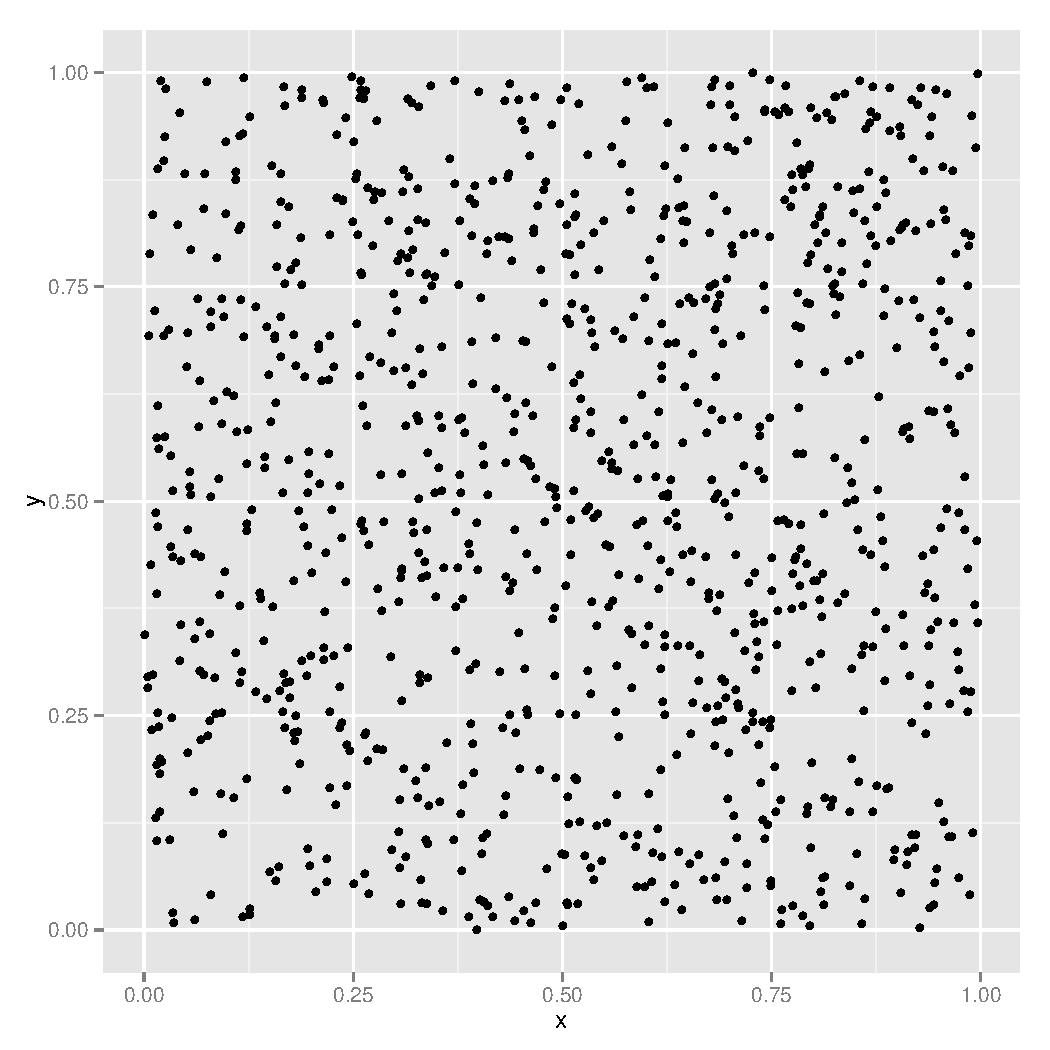
\includegraphics[scale=0.25]{plots/hist.pdf}
  \end{center} 
\end{figure}

\bibliographystyle{plain}
\bibliography{kwow.bib}

\end{document} 
